\section{Optimizers}\label{Optimizers}
It was mentioned at the end of the previous chapter that the recommended optimizers were RMSProp and Adam. RMSProp was used in the experimental set-ups of the Atari games in \cite{DBLP:journals/corr/MnihKSGAWR13} and TORCS in \cite{DBLP:journals/corr/MnihBMGLHSK16}. Also, RMSProp was mentioned in section \ref{RNN} as a solution for the vanishing and exploding gradients problems in RNNs. The Adam optimizer was more often found in the working examples online: in the DDPG for TORCS \cite{DDPG_Torcs}, and in the A3C for Doom \cite{A3CDoom}.

RMSProp and Adam algorithms are extensions of the basic SGD (described in the section \ref{Approximate solution methods}). The problem of identifying a learning rate persists, as it is well known that a too low learning rate results in slow training, whereas a too big learning rate would cause a lot of noise in the objective function so that it would never converge. Not only the speed of training is an indicator of a good learning rate, but also the plotted loss function. Usually, if the learning rate is smaller, then the loss function will be smoother, whereas if the learning rate is greater then the loss function will look noisy in the graphs. These SGD extensions try to solve the learning rate problem by adapting it for each of the parameters.

RMSProp's "idea is to divide the learning rate for a weight by a running average of the magnitudes of recent gradients for that weight" \cite{RMSProp}. The update formula is given by \cite{DBLP:journals/corr/MnihBMGLHSK16}:
\begin{equation}\label{RMSPropUpdate}
\begin{aligned}
g&=\alpha g + (1-\alpha)\Delta \theta^2\\
\theta & \leftarrow \theta - \eta  \frac{\Delta \theta}{\sqrt{g+\epsilon}},
\end{aligned}
\end{equation}
where $\theta$ represents the weights shared across all threads, $\Delta \theta$ is the accumulated gradients of the loss with respect to the $\theta$, $\eta$ is the learning rate, $\alpha$ is the momentum that keeps knowledge of the previous experience, and $g$ is "the moving average of element-wise squared gradients" \cite{DBLP:journals/corr/MnihBMGLHSK16}.

Adam optimizer's principles are a lot like those of RMSProp. Adam algorithm not only keeps the second order moments $g_{t}$, but it also keeps the first order moments $m_{t}$ of the gradients, which are both decayed over time \cite{Optimizers}. The corresponding formulas are listed below:
\begin{equation}\label{Adam}
\begin{aligned}
m_{t+1}&=\alpha_{1} m_{t} + (1-\alpha_{1})\Delta \theta\\
g_{t+1}&=\alpha_{2} g_{t} + (1-\alpha_{2})\Delta \theta^2\\
\hat{m}_{t+1}&=\frac{m_{t+1}}{1-\alpha_{1}^{t+1}}  \\
\hat{g}_{t+1}&=\frac{g_{t+1}}{1-\alpha_{2}^{t+1}}  \\
\theta \leftarrow & \theta - \eta  \frac{\hat{m}_{t+1}}{\sqrt{\hat{g}_{t+1}+\epsilon}}
\end{aligned}
\end{equation}

According to the paper \cite{DBLP:journals/corr/MnihBMGLHSK16}, for the asynchronous deep RL methods like the case of A3C, the RMSProp optimizer with shared weights between threads is more robust and also reduces memory requirements than per-thread weights method. So, shared statistics were used for all the scenarios.

Both RMSProp and Adam optimizers are available in the tensorflow library, and, therefore, were easily tried out and analyzed for the current project, A3C TORCS. A comparison of the two optimizers will be elaborated next, based on the tensorboard graphs generated while training the ANN.

The Figure \ref{fig:OptimizersReward} illustrates the difference in performance between RMSProp and Adam optimizers at the same learning rate of $10^{-5}$, and it also shows the performance of the best learning rate of $10^{-4}$. The x-axis represents the time-steps, and the y-axis represents the value of the accumulated reward.
\begin{figure}[H]
	\centering
	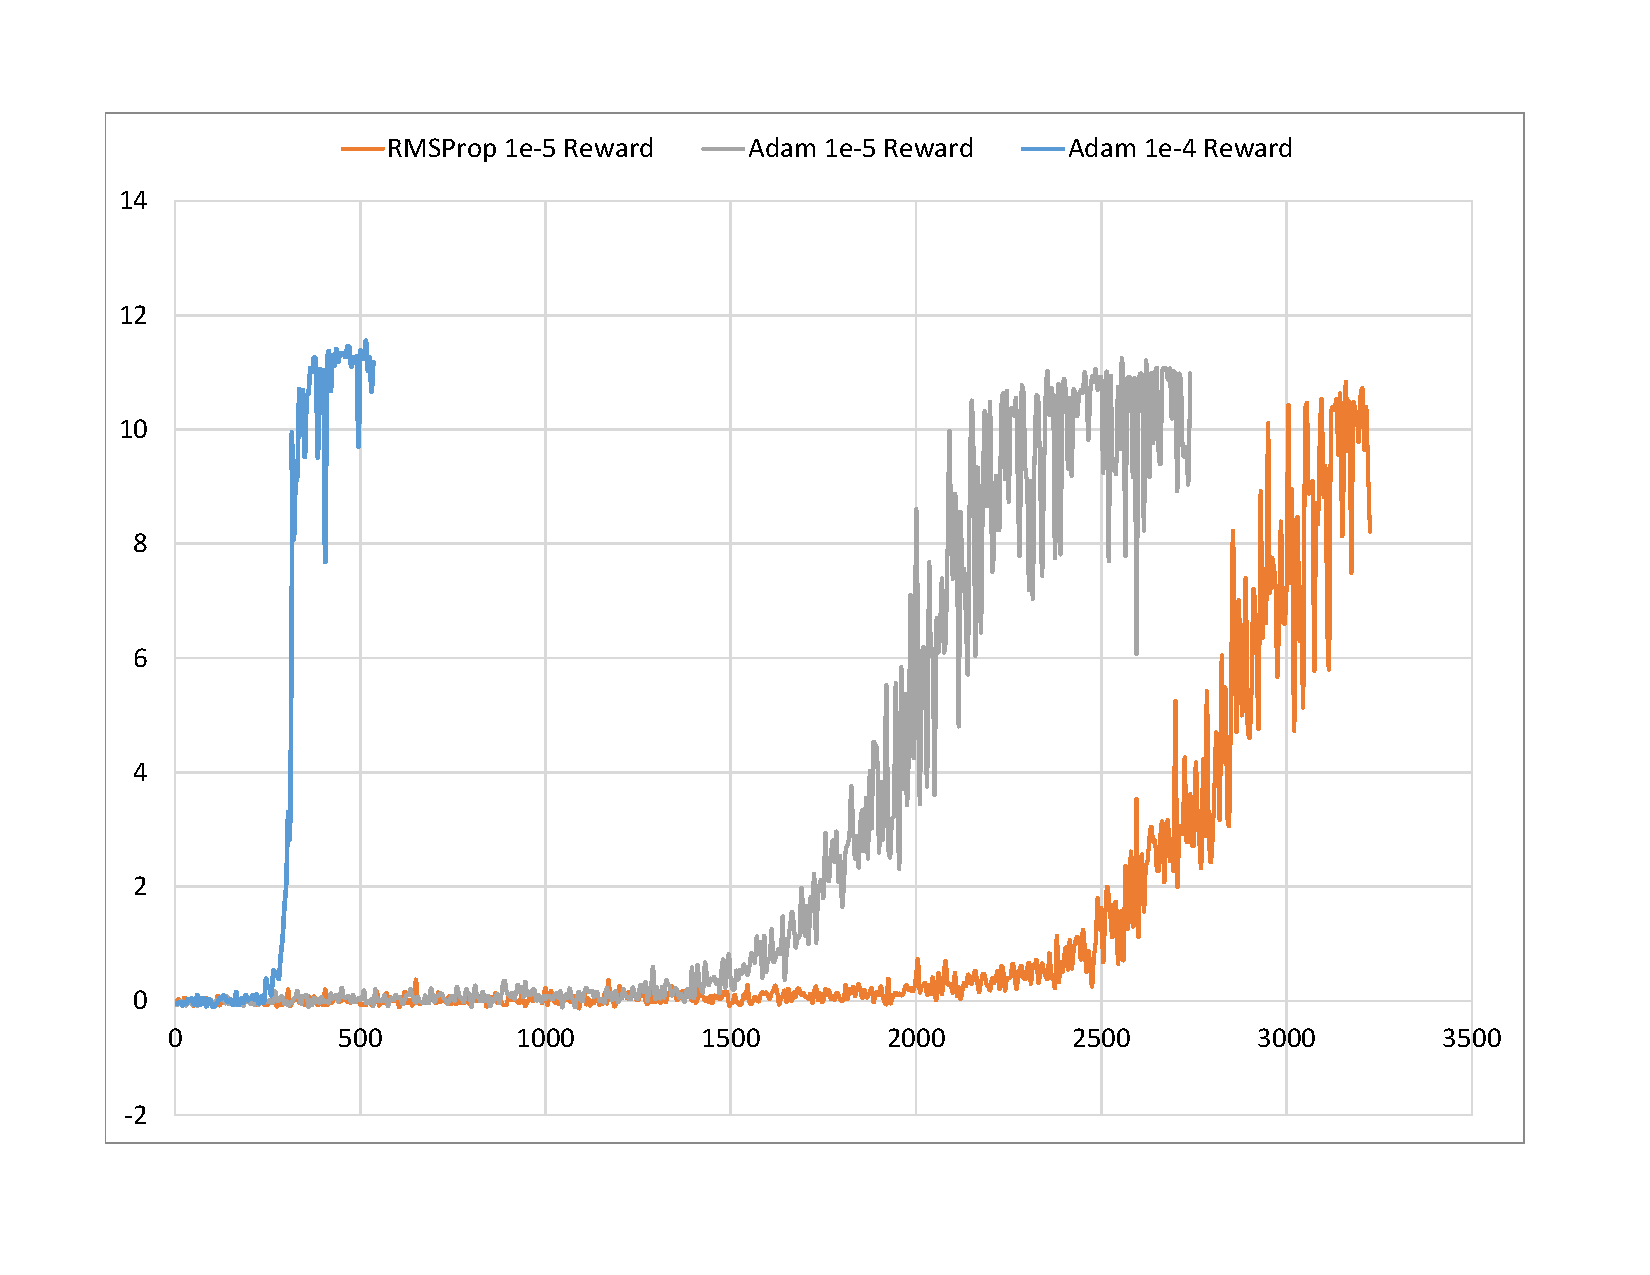
\includegraphics[width=\textwidth]{Figures/OptimizersReward}
	\caption{RMSProp vs. Adam at learning rate $10^{-5}$; and $10^{-5}$ vs. $10^{-4}$ Adam learning rates}
	\label{fig:OptimizersReward}
\end{figure}
From the Figure \ref{fig:OptimizersReward} it is possible to infer that the Adam optimizer is performing better that the RMSProp, because it reaches the total reward of $10$ after around 2.500k steps, while the RMSProp reaches it after around 3.200k steps.

The optimizers were also tried out with different learning rates, and it turned out that the best learning rate for the Adam optimizer is $10^{-4}$, which converges the fastest to the best solution. It is possible to see in the graph that only after 320 steps it started to converge to the optimal solution. Learning rates higher that $10^{-4}$ have been tried out as well, and it was possible to see that the training would never converge, whereas learning rates lower than $10^{-5}$ would slow the training much more.